\documentclass[aspectratio=169]{beamer}
\usepackage[ngerman]{babel}
\usepackage{inputenc}
\usepackage[T1]{fontenc}
\usepackage{lmodern}
\usepackage{listings}
\usepackage{xcolor}
\usepackage{apacite}
\usepackage[percent]{overpic}


\bibliographystyle{apacite}


\definecolor{codegreen}{rgb}{0,0.6,0}
\definecolor{codegray}{rgb}{0.5,0.5,0.5}
\definecolor{codepurple}{rgb}{0.58,0,0.82}
\definecolor{backcolour}{rgb}{0.95,0.95,0.92}
\definecolor{TUCgreen}{cmyk}{1,0,0.9,0.2}

\lstdefinestyle{mystyle}{
    backgroundcolor=\color{backcolour},   
    commentstyle=\color{codegreen},
    keywordstyle=\color{magenta},
    numberstyle=\tiny\color{codegray},
    stringstyle=\color{codepurple},
    basicstyle=\ttfamily\footnotesize,
    breakatwhitespace=false,         
    breaklines=true,                 
    captionpos=b,                    
    keepspaces=true,                 
    numbers=left,                    
    numbersep=5pt,                  
    showspaces=false,                
    showstringspaces=false,
    showtabs=false,                  
    tabsize=2
}

\lstset{style=mystyle}

\graphicspath{{figs/}}

    \usetheme{TUC2}
  %  \usefonttheme{structureitalicserif}
    \setbeamercovered{transparent}

\newcommand{\rhomath}{\( \mathrm{\rho} \)}

\mode<presentation>
    \title{Neural Network-based Detection of Taylor Vortices in Annular Flow Systems}
    \subtitle{Exposé for Master Thesis - Initial Presentation}
    \author{\textbf{Mahyar Alikhani}}
    \institute{Institute of Applied Mechanics}
    \date{\today}

% \setbeamerfont{framesubtitle}{size=\normalfont\tiny}
%%%%%%%%%%%%%%%%%%%%%%%%%%%%%%%%%%%%%%%%%%%%%%%%%%%%%%
\begin{document}
\begin{frame}
\titlepage
% Collaborators: \footnotesize{
%   Stefan Wittek$^1$, Jendrik-Alexander Tr\"oger$^2$, Stefan Hartmann$^2$, Andreas Rausch$^1$
%      }
\end{frame}
%%%%%%%%%%%%%%%%%%%%%%%%%%%%%%%%%%%%%%%%%%%%%%%%%%%%%%

\begin{frame}
\frametitle{Contents}
\tableofcontents
\end{frame}

%%%%%%%%%%%%%%%%%%%%%%%%%%%%%%%%%%%%%%%%%%%%%%%%%%%%%%
\section{Problem Statment}
\begin{frame}
  \frametitle{Problem Statment}
  \large \color{TUCgreen}\textbf{Taylor-Couette Flow}
  \begin{itemize}
    \item It is defined as a fluid dynamic phenomenon that occurs when a fluid is passing between two coaxial-rotating cylinders.
    \item Inner cylinder is typically rotating faster than outer cylinder. This configuration can lead to various flow patterns and instabilities.
    \item Dimensionless control parameters like \(\mathnormal{Re}\), ration of cylinder radii, 
  \end{itemize}
\end{frame}

%%%%%%%%%%%%%%%%%%%%%%%%%%%%%%%%%%%%%%%%%%%%%%%%%%%%%%
\section{Task definition and objective}
\begin{frame}
  \frametitle{Objectives}
  \begin{itemize}
    \item Governing equ:\\
      \begin{equation}
        \frac{\partial \mathbf{u}}{\partial t} + (\mathbf{u} \cdot \nabla)\mathbf{u} = -\frac{1}{\rho}\nabla p + \nu \nabla^2 \mathbf{u} + \mathbf{f}
      \end{equation}
    \item w.r.t boundary conditions:\\
    \begin{align}
      \mathbf{u} &= \mathbf{u}_0 \quad \text{at} \quad \Gamma_1 \\
      \mathbf{u} &= 0 \quad \text{at} \quad \Gamma_2 \\
      \frac{\partial p}{\partial n} &= 0 \quad \text{at} \quad \Gamma_3
    \end{align}

  \end{itemize}
\end{frame}
%%%%%%%%%%%%%%%%%%%%%%%%%%%%%%%%%%%%%%%%%%%%%%%%%%%%%%
\section{Litrature Review}
\begin{frame}
  \frametitle{Litrature Review}
  \begin{itemize}
    \item[(a)]  \cite{Liang2018}, a CNN-based vortex identification method to use both local and global information of flow field.
  \end{itemize}
  \begin{center}
    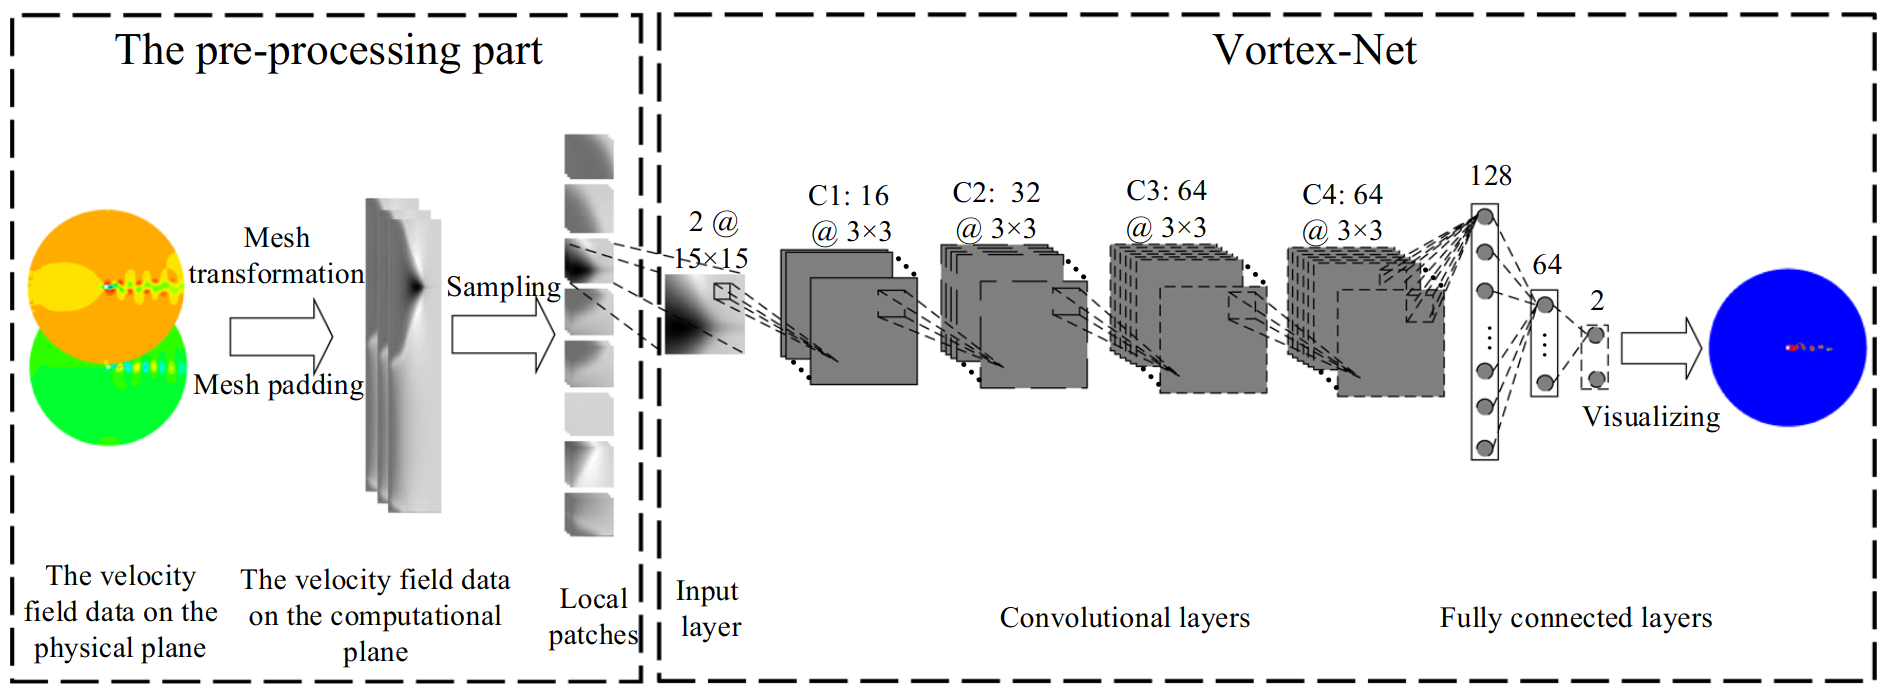
\includegraphics[width=0.85\textwidth]{paper_review.png}
  \end{center}
\end{frame}

%%%%%%%%%%%%%%%%%%%%%%%%%%%%%%%%%%%%%%%%%%%%%%%%%%%%%%
\begin{frame}
  \frametitle{Litrature Review}
  \begin{itemize}
    \item[(b)] \cite{Wang2021}, replacing the fully-connected NN with a segmented network to reduce the computational complexity.
  \end{itemize}
  \begin{center}
    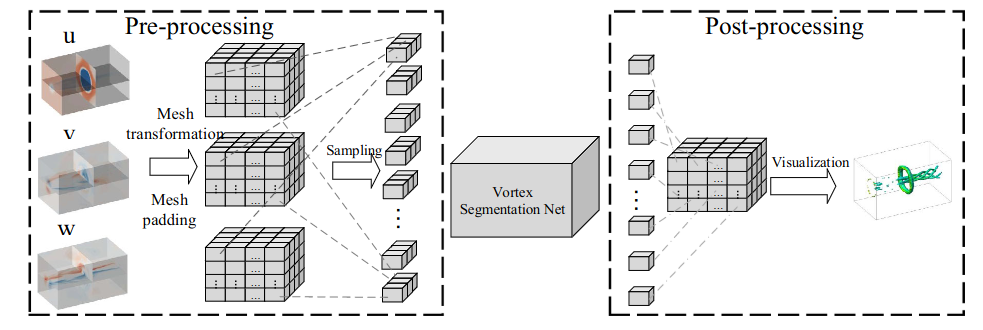
\includegraphics[width=0.85\textwidth]{litratur_review_wang.png}
  \end{center}
\end{frame}


%%%%%%%%%%%%%%%%%%%%%%%%%%%%%%%%%%%%%%%%%%%%%%%%%%%%%%
\section{Approache}
\begin{frame}
  \frametitle{Approaches}
  \begin{itemize}
    \item The 
  \end{itemize}
\end{frame}
%%%%%%%%%%%%%%%%%%%%%%%%%%%%%%%%%%%%%%%%%%%%%%%%%%%%%%
\begin{frame}
  \frametitle{Results}
  \begin{minipage}{0.55\textwidth}
    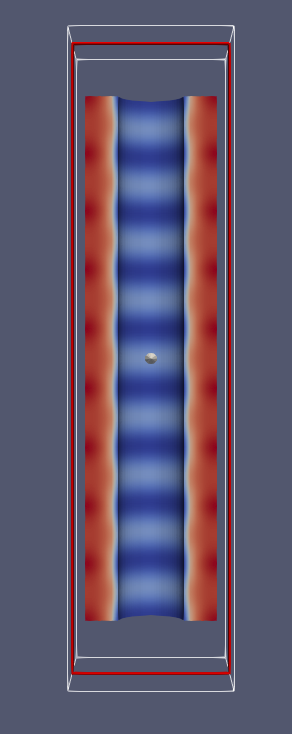
\includegraphics[width=0.30\textwidth, trim={0cm 0cm 0cm 0cm}, clip]{Taylor-couette.png}
  \end{minipage}
\end{frame}

%%%%%%%%%%%%%%%%%%%%%%%%%%%%%%%%%%%%%%%%%%%%%%%%%%%%%%
%\begin{frame}
%\frametitle{}\
%  \begin{minipage}{0.45\textwidth}
%    \centering
%    %(A) Global ---> Global
%    \vfill
%    %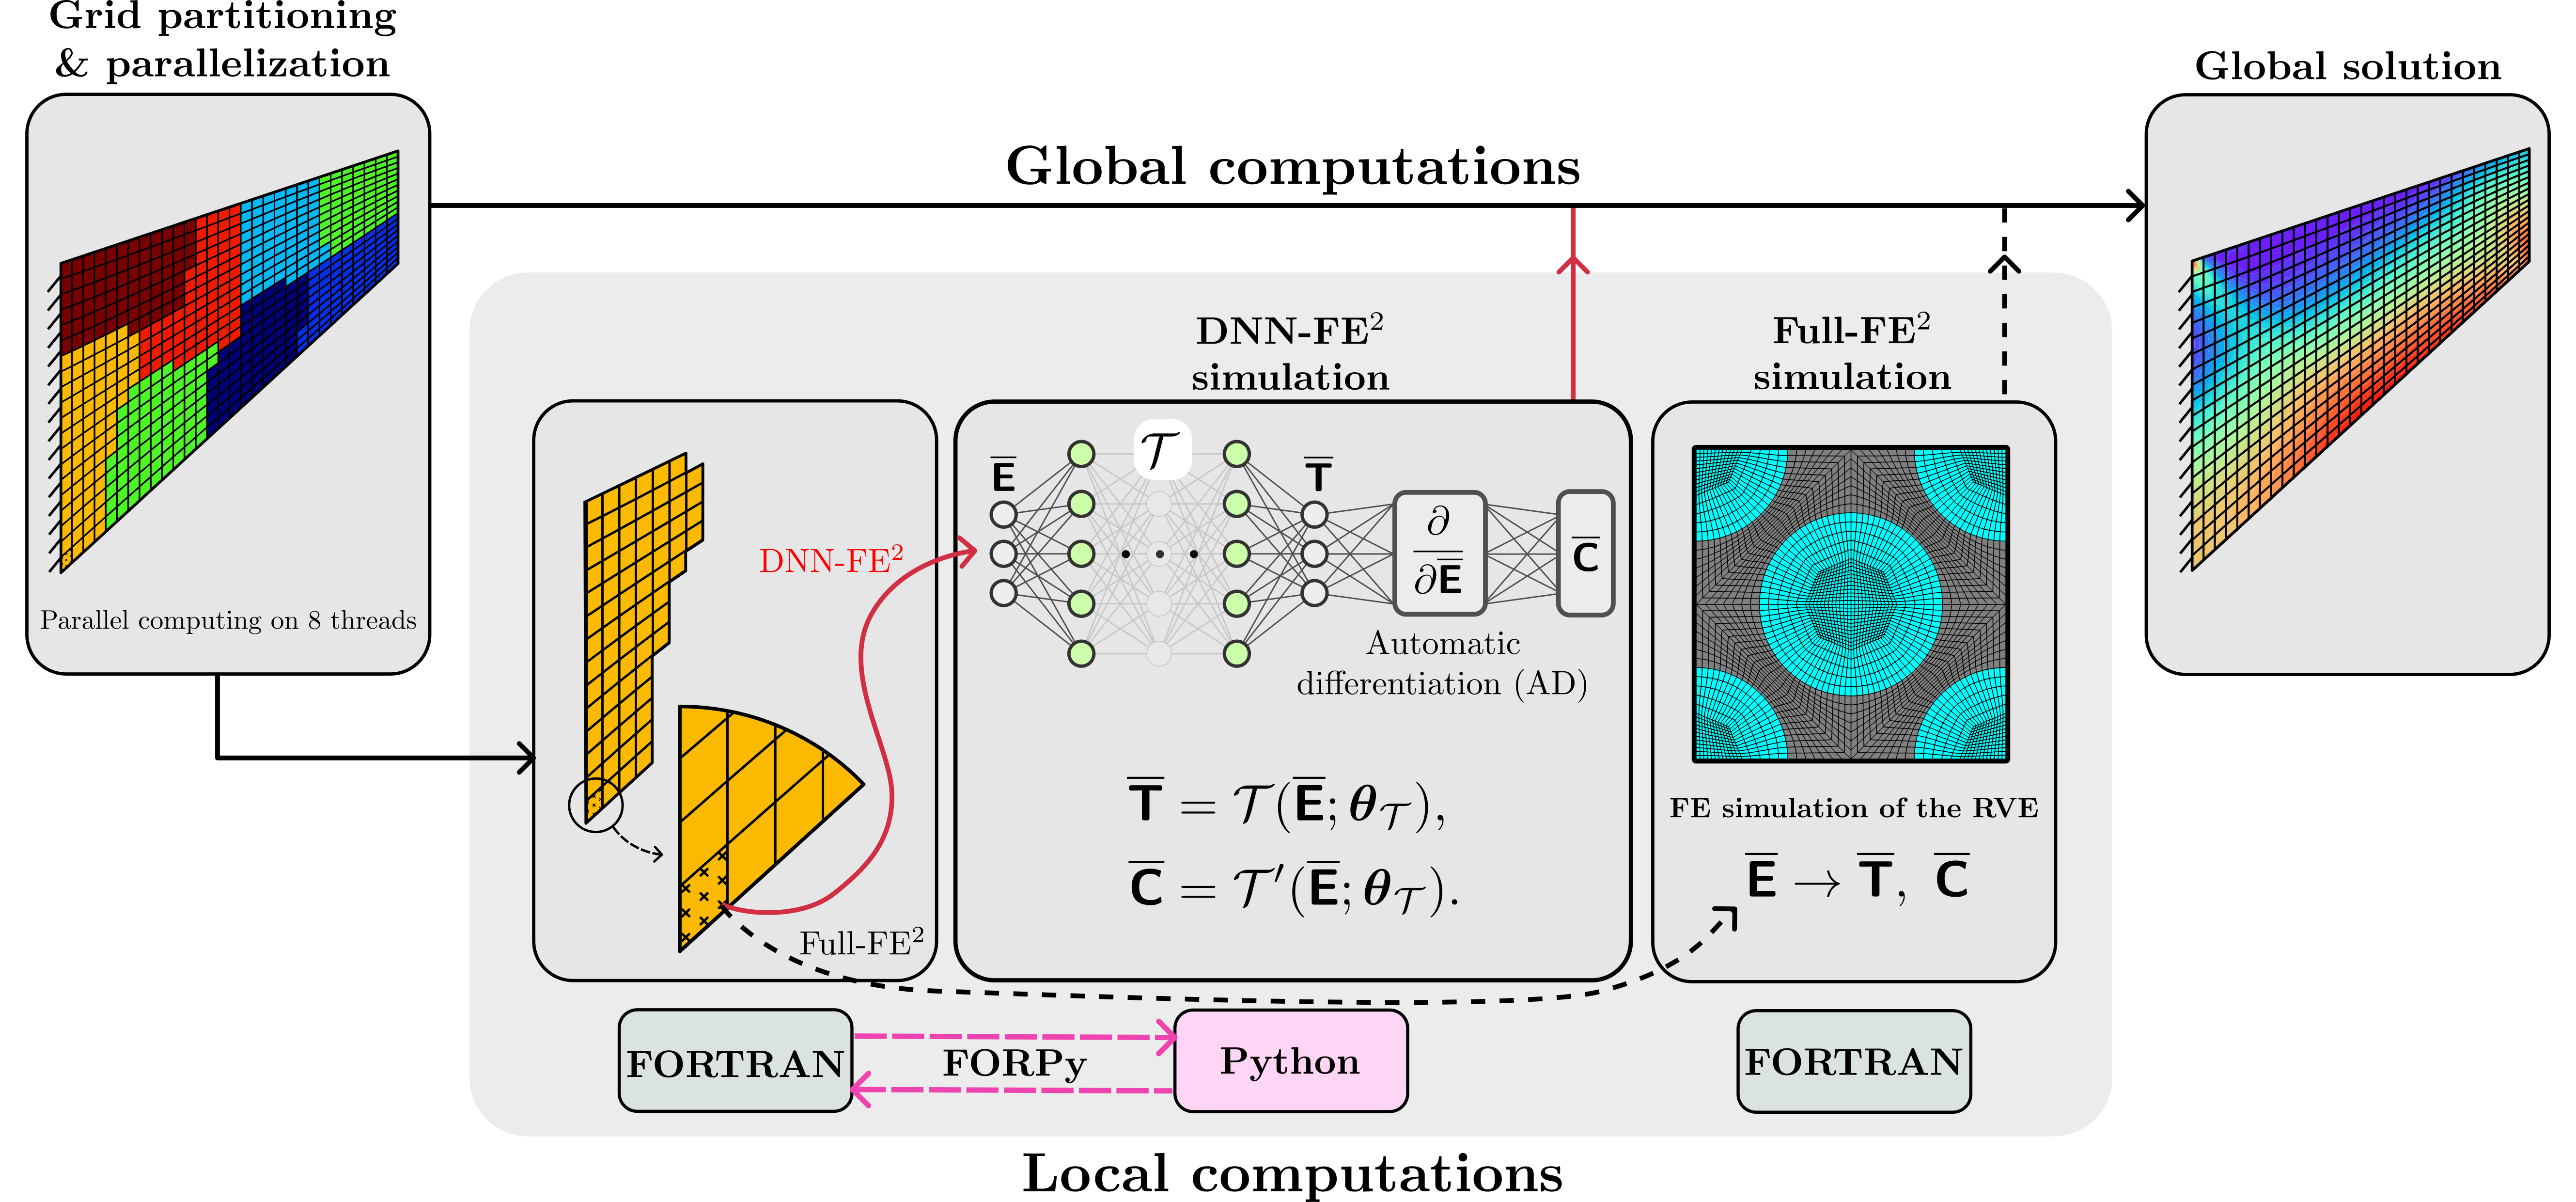
\includegraphics[width=0.9\textwidth, trim={10cm 2.3cm 9.9cm 4.2cm}, clip]{drawing}
%  \end{minipage}
%  \begin{minipage}{0.45\textwidth}
%    \centering
%    %(B) Global ---> Local ---> Global
%    \vfill
    %\hfill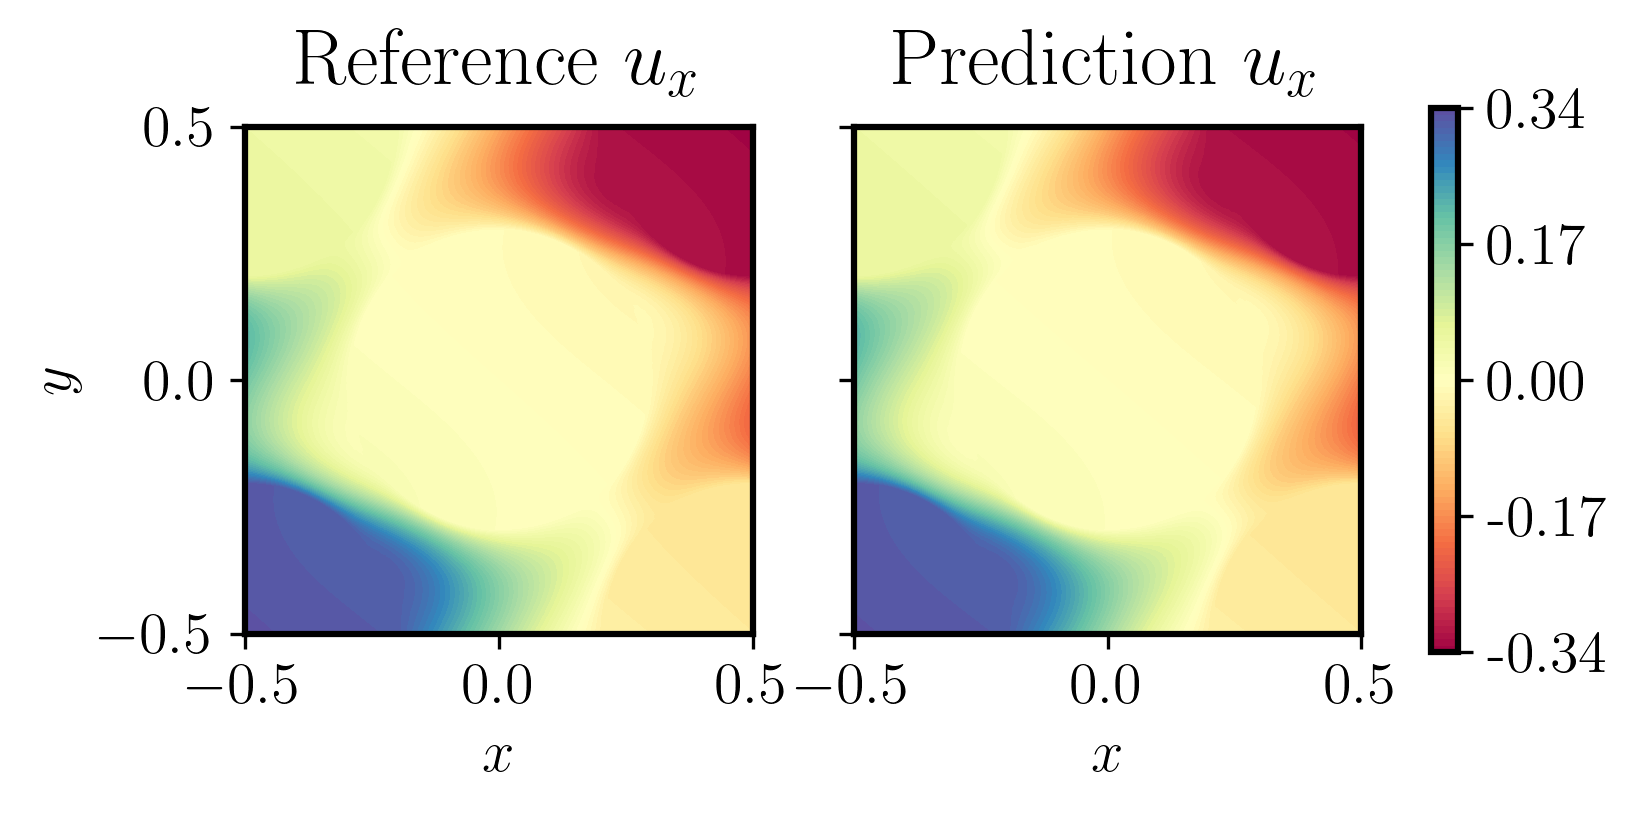
\includegraphics[width=0.95\textwidth, trim={0cm 0cm 7cm 0cm}, clip]{rve1_ux.png}
%  \end{minipage}
%\end{frame}


%%%%%%%%%%%%%%%%%%%%%%%%%%%%%%%%%%%%%%%%%%%%%%%%%%%%%%

\begin{frame}
  \frametitle{}\
  
\begin{minipage}{0.3\textwidth}
    %Inputs of branch: \\$\mathbf{E} \in \mathbb{R}^3$, ($N_s$, 3)

    %Outputs of branch: \\$\boldsymbol{b} \in \mathbb{R}^{N_f}$, ($N_s$, $N_f$)

    \vspace{\baselineskip}

    %Inputs of trunk: \\$\mathbf{X} \in \mathbb{R}^{10561}$, (10561, 2)

    %Outputs of trunk: \\$\boldsymbol{t} \in \mathbb{R}^{N_f}$, (10561, $N_f$)
\end{minipage}
\begin{minipage}{0.35\textwidth}
    %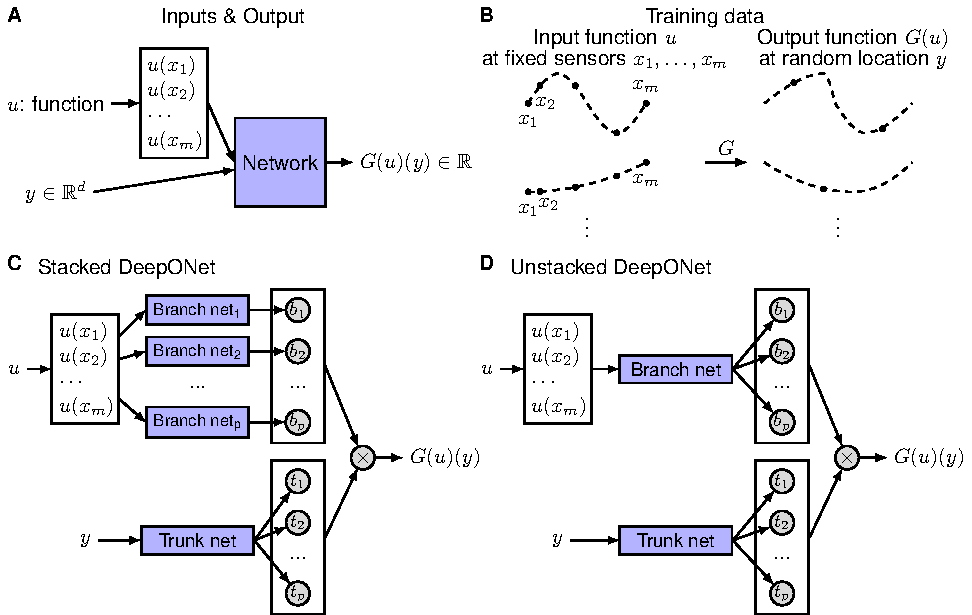
\includegraphics[width=\textwidth, trim={10.05cm 0cm 0cm 4.8cm}, clip]{deeponet.pdf}
\end{minipage}
\begin{minipage}{0.3\textwidth}

  %Outputs: \\$\boldsymbol{u} \in \mathbb{R}^{2\times10561}$, \\($N_s$, $N_f$) $\bigotimes$ (10561, $N_f$)$^{T}$

\end{minipage}
\end{frame}


\section{Time Planning}
\begin{frame}
  \frametitle{Timeline}
  \begin{center}
    \begin{figure}
      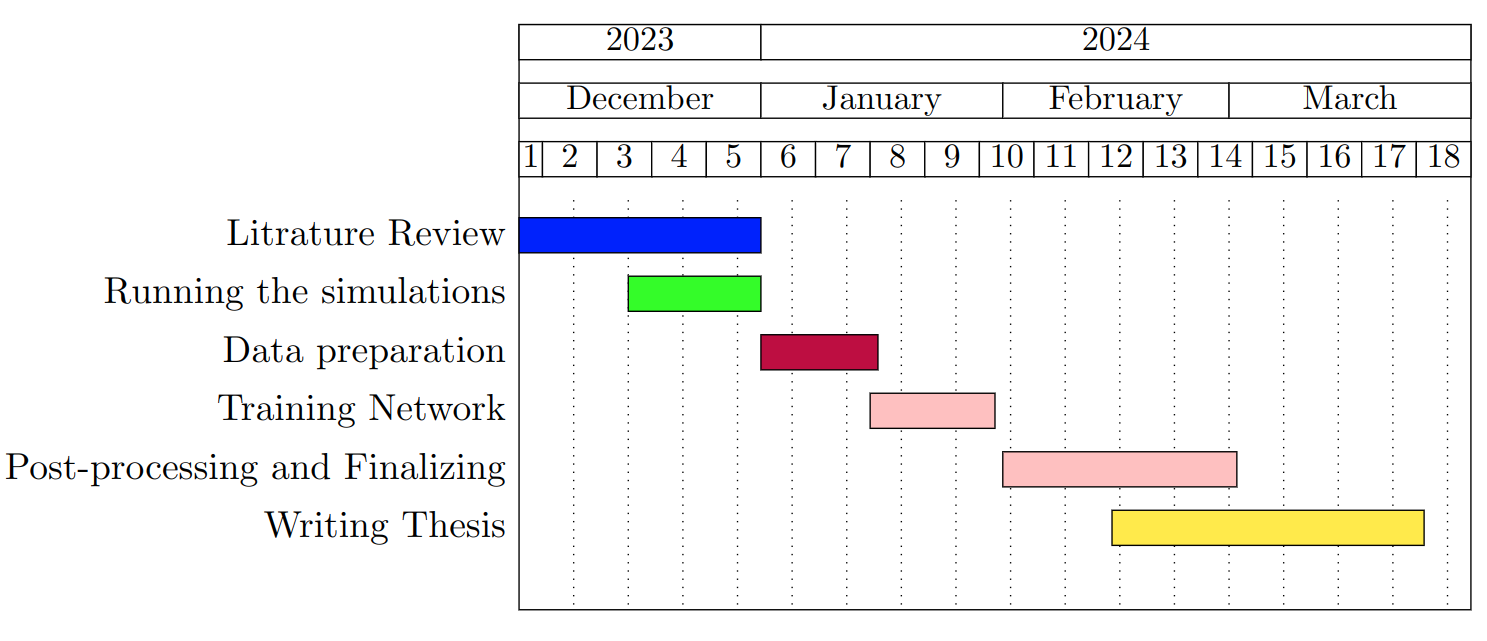
\includegraphics[width=0.9\textwidth]{figs/Timeplan.png}
      \caption{Timeplan}
    \end{figure}
  \end{center} 
\end{frame}

\begin{frame}
  % \centering
  \begin{minipage}{0.1\textwidth}
    \hfill
  \end{minipage}
  \begin{minipage}{0.89\textwidth}
    \color{TUCgreen}{\textbf{\Large{Thank you!}}}\\
  \color{black}{
  \small{Any questions?}
  }
  \end{minipage}
  
\end{frame}

\bibliography{references.bib}

\end{document}

